\vspace*{8.5cm}

\begin{flushright}
	\section{\huge{\underline{Project Description}}}
\end{flushright}

		\subsection{Introduction}
			Enter some text here.
			
		\subsection{Hardware}
			\subsubsection{MCU}
				The \textsc{led matrix} is built around a ATmega328P AVR microcontroller. This MCU is based on advanced RISC architecture, 8 bit MCU and 23 programmable I/O lines. For controlling the \textsc{led matrix} shift registers are used, 2 for Column and 1 for row, due to shift registers few MCU I/O lines are used.
			\subsubsection{LED Matrix}
				 Single colour  RED 5mm LEDs used to build the matrix, total of 128 LEDs required for 16x8 matrix. An array of transistors configured as switch to provide required current for each row of LED matrix.  
				
			\subsubsection{Power supply}
				The project utilises a transformerless capacitive power supply design. Such a design is helpful in reducing the overall cost of project and also utilises fewer components thus saving space and cost.
			\subsubsection{Input}
				 The project is aimed to dynamically modify the display commands through an input source like PC or BLE. Such a feature helps in modifying the display at will rather than modifying the source code.
				 
			\begin{figure}[H]
					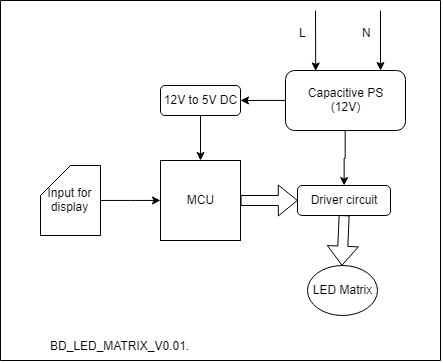
\includegraphics[scale=01]{BD_LED_MATRIX_V1.png}
					\caption{Block Diagram V0.01}
					\label{fig:image1}
			\end{figure}
				  



